\chapter{Diseño del Videojuego (GDD) y Dirección Artística}

Este capítulo recoge la especificación completa del diseño del juego, incluyendo la sinopsis, los mundos abstractos, las reglas del sistema adaptativo, el consentimiento del jugador y el documento de diseño artístico, que abarca el estilo visual, la paleta de colores, el diseño de personajes y entornos, la iluminación y la interfaz de usuario (UI) adaptativa. La justificación de las decisiones de diseño se fundamenta en la investigación documental y en el asesoramiento psicológico recibido durante la fase de desarrollo del proyecto, así como en la experiencia adquirida a lo largo del Grado en Ingeniería Multimedia. Además, se incluyen referencias a obras de videojuegos independientes y experimentales que han servido como inspiración para la creación de este prototipo funcional. Y como parte de la documentación del GDD, se presentan diagramas de flujo y tablas que ilustran la evolución de los perfiles conductuales del jugador y su impacto en la jugabilidad, así como la relación entre los elementos narrativos y las mecánicas adaptativas implementadas en el juego. En las referencias bibliográficas se incluyen fuentes académicas y artículos especializados que respaldan las decisiones de diseño y la implementación de mecánicas adaptativas en videojuegos, así como estudios sobre narrativa interactiva, salud mental y representación de género en medios digitales ya que estos aspectos son fundamentales para la comprensión del contexto y la relevancia del proyecto porque permiten situar el prototipo dentro de un marco teórico sólido y ofrecer una experiencia de juego que sea significativa y respetuosa con la temática abordada.

\section{Concepto General y Sinopsis Argumental}
Título del Proyecto: Sin definir
Género: aventura narrativa 2D / Exploración introspectiva
Plataforma Objetivo: PC / Mac (Entorno Unity)
Público Objetivo: jugadores interesados en experiencias narrativas independientes, representación LGTBIQ+, salud mental y diseño de juego experimental.

\subsection{Sinopsis}
El juego sitúa al personaje protagonista en el centro de un colapso apocalíptico. Lo que a primera vista aparenta ser la destrucción física de un mundo urbano decadente revela ser la representación externa del agotamiento mental causado por la disforia, la imposición de roles de género y el rechazo social acumulado. Para sobrevivir, el protagonista debe atravesar una serie de planos abstractos que personifican las etapas de su conflicto identitario, enfrentándose a manifestaciones físicas del escrutinio social y aprendiendo a reconocer su propio espacio e identidad.

\section{Diseño Narrativo y Estructura de Mundos Abstractos}
El desarrollo narrativo del juego se formula a través de tres mundos o dimensiones abstractas principales, cada una vinculada a un estado emocional y a un conjunto de estresores concretos:
\begin{itemize}
  \item Mundo 1: Vecindad Urbana: estructuras monolíticas, sombras fijas y entornos vacíos de vida. Simboliza la presión del entorno social y la necesidad forzada de adaptarse a expectativas externas. Las mecánicas iniciales son rígidas y restrictivas. Aquí el protagonista se enfrentará a dos manifestaciones abstractas: un ángel ciego y herido, y una entidad de la oscuridad sin cuerpo físico.
  \item Mundo 2: Laberinto Fracturado: escenarios fragmentados, flotantes, caracterizados por geometrías inestables y ecos sonoros, creando un especie de laberinto complicado. Representa la fase más crítica del agotamiento psicológico e internalizado. Aquí es donde el sistema adaptativo empieza a sugerir mutaciones profundas en el control del personaje y se enfrenta a dos manifestaciones abstractas: un amigo olvidado el cual busca que le encuentren, y un reflejo mutado del propio protagonista.
  \item Mundo 3: Azotea Libre: un plano de líneas depuradas, iluminación suave y espacio amplio. Esta etapa final es el desenlace que se adapta para ofrecer una resolución abierta cuyo tono e interpretación dependerá del perfil conductual consolidado a lo largo del juego. Aquí únicamente se dialogará directamente con el protagonista.
\end{itemize}

\section{Sistema de Mecánicas Adaptivas y Perfiles de Jugador}
El núcleo interactivo reside en la clasificación implícita de las acciones del jugador en tres perfiles conductuales:
\begin{itemize}
  \item Agresivo: realiza a menudo acciones de confrontación directa contra los obstáculos/enemigos, junto con un avance rápido seguido y uso frecuente de habilidades de impacto.
  \item Pasivo: se encuentra en largos periodos de inmovilidad ante la presencia de enemigos, avance lento, interacción cuidadosa con el entorno y casi nunca usa habilidades de impacto.
  \item Evasivo: uso constante de saltos, esquivas y rodeos para evitar contacto con posibles amenazas, teniendo una mínima interacción directa con el entorno.
\end{itemize}
A continuación, se muestra un esquema de flujo del sistema de mecánicas adaptativas:
\begin{figure}[H]
  \centering
  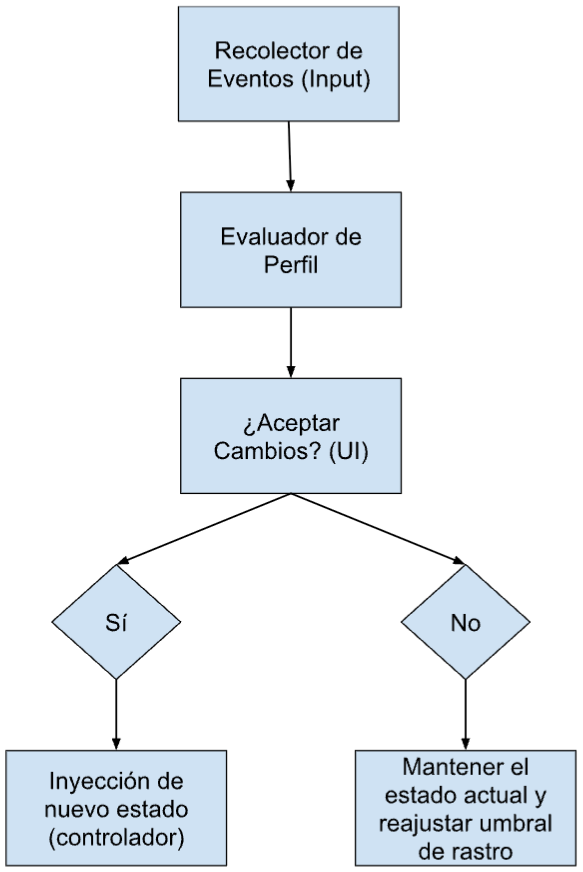
\includegraphics[width=0.8\textwidth]{Esquema.png}
  \caption{Esquema de flujo del sistema de mecánicas adaptativas}
  \label{fig:esquema-mecanicas}
  \fuente{elaboración propia}
\end{figure}
%lista de habilidades y transformaciones.
%NO ESTOY MUY SEGURO CON EL TEMA DE PERFILES, PUEDE ESTAR SUJETOS A CAMBIOS PEQUEÑOS O GRANDES.

\section{Consentimiento del Jugador y Accesibilidad Emocional}
A diferencia de otros títulos con sistemas de adaptabilidad oculta que modifican las reglas unilateralmente, este juego introduce la mecánica del Consentimiento Explícito. De tal manera que, cuando el analizador detecta un hábito consolidado a partir de las acciones optadas por el jugador, el juego presenta una notificación en pantalla donde el jugador puede seleccionar si aceptar la mutación de sus habilidades (por ejemplo, transformar esquivar en una carga frontal) o rechazar el cambio, conservando la configuración de control previa. Esta decisión garantiza que la agencia del usuario no sea vulnerada y evita la frustración mecánica, reforzando la idea de que la persona al mando tiene el control sobre el proceso de afrontamiento de su personaje.

\section{Documento de Diseño Artístico}
\subsection{Estilo Visual y Paleta de Colores}
La dirección artística opta por un estilo 2D con una marcada sensación de profundidad tridimensional (2.5D), articulado desde una perspectiva en tercera persona cenital oblicua (\textit{top-down} 3/4). Este enfoque visual toma como referentes principales la disposición espacial de \textit{Undertale} \parencite{fox2015}, junto con el acabado pictórico, atmosférico y estilizado de obras como \textit{Oxenfree} \parencite{nightschool2016} y \textit{Night in the Woods} \parencite{infinitefall2017}. De este modo, se evita el \textit{pixel art} convencional para construir entornos transitables en todas las direcciones del plano ($X$ e $Y$) que envuelven físicamente al protagonista.
\\\\
Esta identidad visual se fundamenta en tres pilares expresivos que refuerzan la metáfora del agotamiento psicológico y la crisis de identidad de género:
\begin{itemize}
  \item La cámara en ángulo picado oblicuo permite al jugador desplazarse libremente hacia el fondo, el frente y los laterales del escenario. A diferencia de una vista lateral plana, esta perspectiva subraya la vulnerabilidad del personaje al situarlo rodeado por la arquitectura opresiva y las manifestaciones del escrutinio social.
  \item Las figuras del plano jugable presentan siluetas vectoriales definidas y expresivas, mientras que los pavimentos en perspectiva, las estructuras colapsadas y los abismos emplean texturas orgánicas, pinceladas desgastadas y densos bancos de niebla que acentúan la perspectiva aérea y el aislamiento.
  \item La paleta cromática evoluciona según la carga emocional de la escena y la transición a través de los tres mundos abstractos (Tabla 1):
\end{itemize}
\begin{table}[H]
  \centering
  \caption{Paleta cromática de los entornos abstractos del juego y la evolución del UI.}
  \label{tab:paleta}
  \small
  \renewcommand{\arraystretch}{1.2}
  \begin{tabularx}{\textwidth}{YYYY}
    \toprule
    Entorno/Estado & Tono Dominante & Tono Secundario & Tono de Acento \\
    \midrule
    Mundo 1 &  & & \\
    Mundo 2 &  &  & \\
    Mundo 3 &  &  & \\
    \bottomrule
  \end{tabularx}
  \fuente{elaboración propia.}
\end{table}

\subsection{Diseño de Personajes y Entornos}
En primer lugar, en cuanto al personaje principal presenta un diseño minimalista de líneas fluidas y silueta andróginal, optimizado mediante sprites para asegurar su legibilidad en el plano bidimensional (X e Y) bajo la perspectiva cenital oblicua (top-down ¾). Siguiendo los principios de identificación empática \parencite{navarro2023}, se prescinde de rasgos faciales detallados, concentrando la expresividad en su postura corporal, el movimiento de su vestimenta y su sombra proyectada.
\\\\
Una vez que el jugador acepta un cambio, el aspecto del avatar muta en tiempo real según la Tabla 2
\begin{table}[H]
  \centering
  \caption{Evolución visual del protagonista según el perfil conductual consolidado.}
  \label{tab:EvolucionVisual}
  \small
  \renewcommand{\arraystretch}{1.2}
  \begin{tabularx}{\textwidth}{>{\raggedright\arraybackslash}p{2.5cm}YYY}
    \toprule
    Perfil Conductual & Silueta y Contorno & Animación y Postura Corporal & Tratamiento Cromático y Efectos \\
    \midrule
    Agresivo (Confrontación) & Cortes geométricos angulosos y trazo vectorial más grueso & Postura firme e inclinada hacia adelante en avances e impactos & Alto contraste respecto al pavimento y destellos de impacto\\
    Pasivo (Bloqueo) & Silueta compacta, encogida y de bordes redondeados & Avance lento, hombros retraídos y prenda replegada como refugio & Tonos desaturados que se mezclan con las sombras del entorno\\
    Evasivo (Huida) & Acabado liviano con bordes orgánicos difuminados & Movimiento ágil en saltos, esquivas y rodeos constantes & Estela traslúcida al cambiar rápidamente de dirección\\
    \bottomrule
  \end{tabularx}
  \fuente{elaboración propia.}
\end{table}

En segundo lugar, aplicando los principios de la narrativa ambiental \parencite{finestrat2018}, los escenarios y las entidades que los habitan proyectan el conflicto interno del protagonista sin recurrir a texto expositivo. Para materializar la profundidad tridimensional (2.5D) en Unity mediante \textit{Tilemap} y \textit{Sprite Editor} \parencite{unity2023}, cada escena combina un primer plano oclusivo (\textit{foreground}), un plano medio jugable con ordenación dinámica en el eje vertical (\textit{Y-Sorting}, permitiendo al avatar rodear obstáculos por delante y por detrás), y un fondo abisal con desplazamiento diferencial (\textit{parallax}).
\\\\
La distribución espacial de los tres mundos y el diseño de sus respectivas manifestaciones abstractas se organizan en la Tabla 3:
\begin{table}[H]
  \centering
  \caption{Diseño escenográfico y manifestaciones abstractas por mundos.}
  \label{tab:DiseñoEscenografico}
  \small
  \renewcommand{\arraystretch}{1.2}
  \begin{tabularx}{\textwidth}{>{\raggedright\arraybackslash}p{2.5cm}YYY}
    \toprule
    Entorno/Estado & Distribución espacial y recursos en Unity (2.5D) & Manifestaciones abstractas & Diseño visual de las manifestaciones \\
    \midrule
    Mundo 1 & Calles y plazas delimitadas por estructuras monolíticas y sombras fijas (Tilemap estático) & Ángel ciego y herido;Entidad de la oscuridad& El ángel emplea trazos vectoriales rígidos y agrietados; la entidad utiliza un espacio completamente oscuro sin contorno fijo desde donde únicamente se muestran sus manos\\
    Mundo 2 & Islas flotantes y geometrías inestables suspendidas sobre abismos (Parallax multicapa) & Amigo olvidado;Reflejo mutado del protagonista& El amigo presenta una silueta fragmentada y brumosa; el reflejo distorsiona el sprite del protagonista con proporciones quebradas\\
    Mundo 3 & Explanada amplia y despejada de líneas depuradas sin obstáculos restrictivos & Protagonista (diálogo interno) & Espacio abierto enfocado exclusivamente en la figura del propio avatar\\
    \bottomrule
  \end{tabularx}
  \fuente{elaboración propia.}
\end{table}

\subsection{Iluminación y Diseño de Interfaz (UI) Adaptativa}
En cuanto a la iluminación, para dotar al entorno cenital oblicuo (\textit{top-down} 3/4) de volumen sin sobrecargar el rendimiento ni complicar la jerarquía de Unity, se emplea el sistema \textit{2D Lighting} del paquete \textit{Universal Render Pipeline} (\ac{URP} 2D) \parencite{unity2023}, de tal manera que:
\\\\
Por un lado, en lugar de sistemas lumínicos dinámicos complejos, utilizan luces globales suaves (Global Light 2D) combinadas con luces puntuales fijas (Point Lights 2D) en puntos estratégicos de los escenarios para marcar zonas de interés o áreas de transición.
\\\\
Por otro lado, el avatar incorpora un único componente de luz puntual hijo de su jerarquía (Point Light 2D de corto alcance), lo que proyecta un halo circular continuo sobre el suelo a su alrededor sin requerir cálculos pesados de sombras en tiempo real, garantizando una ejecución fluida en el prototipo.
\\\\
En cuanto a la interfaz de usuario (UI) adaptativa se implementa mediante un único lienzo (Canvas) en espacio de pantalla con elemetnos dinámicos controlados por scripst ligeros. La ventana de notificación del Consentimiento Explícito se resuelve mediante un panel de diálogo flotante básico que pausa temporalmente la lógica de movimiento (Time.timeScale = 0), evitando la complejidad de gestionar interfaces completamente diegéticas en 3D.
\\\\
El cambio visual de los elementos de UI según el perfil detectado por el sistema en segundo plano se gestiona de forma eficiente mediante perfiles de datos (ScriptableObjects), adaptando sus parámetros visuales conforme a la Tabla 4:
\begin{table}[H]
  \centering
  \caption{Cambio visual de la interfaz de usuario (UI) según el perfil conductual evaluado.}
  \label{tab:CambioVisualUI}
  \small
  \renewcommand{\arraystretch}{1.2}
  \begin{tabularx}{\textwidth}{>{\raggedright\arraybackslash}p{2.5cm}YYY}
    \toprule
    Perfil conductual & Estilo Visual de la UI & Comportamiento en Pantalla & Nivel de opacidad y contraste \\
    \midrule
    Agresivo & Bordes angulosos y trazos destacados & Posición fija y estable en la esquina superior del lienzo & Opacidad alta y colores contrastados\\
    Pasivo & Líneas finas y formas compactas & Retraimiento visual hacia los márgenes de la pantalla & Opacidad reducida\\
    Evasivo & Trazos suaves y redondeados & Movimiento de flotación sútil adaptado al desplazamiento del avatar & Opacidad variable vinculada a la velocidad de movimiento\\
    \bottomrule
  \end{tabularx}
  \fuente{elaboración propia.}
\end{table}

% El código usa la familia de ancho fijo (código~\ref{lst:ejemplo}).
% \begin{lstlisting}[language=Java, caption={Ejemplo de función}, label={lst:ejemplo}]
% // Calcula la distancia entre dos puntos
% public double distancia(Punto a, Punto b) {
%     double dx = a.x - b.x;
%     double dy = a.y - b.y;
%     return Math.sqrt(dx * dx + dy * dy);
% }
% \end{lstlisting}

% \section{Ejemplo de fórmula}
% Las fórmulas sencillas en línea se escriben así: $x^2 + y^2 = r^2$, $a + b = c$.
% Las más complejas, numeradas:
% \begin{equation}
%   d(a,b) = \sqrt{(a_x - b_x)^2 + (a_y - b_y)^2}
%   \label{eq:distancia}
% \end{equation}
